\documentclass{article}
\usepackage[utf8]{inputenc}
\usepackage[
    %backend=biber, 
    natbib=true,
    style=numeric,
    sorting=none
]{biblatex}
%\usepackage{biblatex} %Imports biblatex package
\addbibresource{literatura.bib} %Import the bibliography file
\usepackage[slovak]{babel}
\usepackage[T1]{fontenc}
\usepackage{amsmath}
\usepackage{fullpage}
\usepackage{graphicx}
\usepackage{txfonts}
\usepackage{gensymb}
\usepackage{eurosym}
\usepackage[export]{adjustbox}
\usepackage[symbol*]{footmisc}
\usepackage{mathtools}
\usepackage{enumitem}
\usepackage[unicode]{hyperref}
\usepackage{epsfig}
\usepackage{indentfirst}
\usepackage{subfig}
\usepackage{hyperref}
\usepackage{tabularx,ragged2e,booktabs,caption}
\usepackage{esvect}
\usepackage{pdfpages}
\usepackage{csquotes}
\usepackage{url}
\usepackage{textcomp}
\usepackage[hypcap = false]{caption}
\usepackage{calc}
\usepackage{graphicx}
\usepackage{color}
\usepackage{wrapfig}
\usepackage{float}
\usepackage{multirow}
\newfloat{graph}{htbp}{grp}
\floatname{graph}{Graf}
%\usepackage{fancyhdr}
%\usepackage[head=12pt]{geometry}
\usepackage[version=4]{mhchem}


\title{P2_XXVI}
\author{Ján Kovačovský}
\date{December 2019}

\begin{document}
\renewcommand{\thefootnote}{\arabic{footnote}}

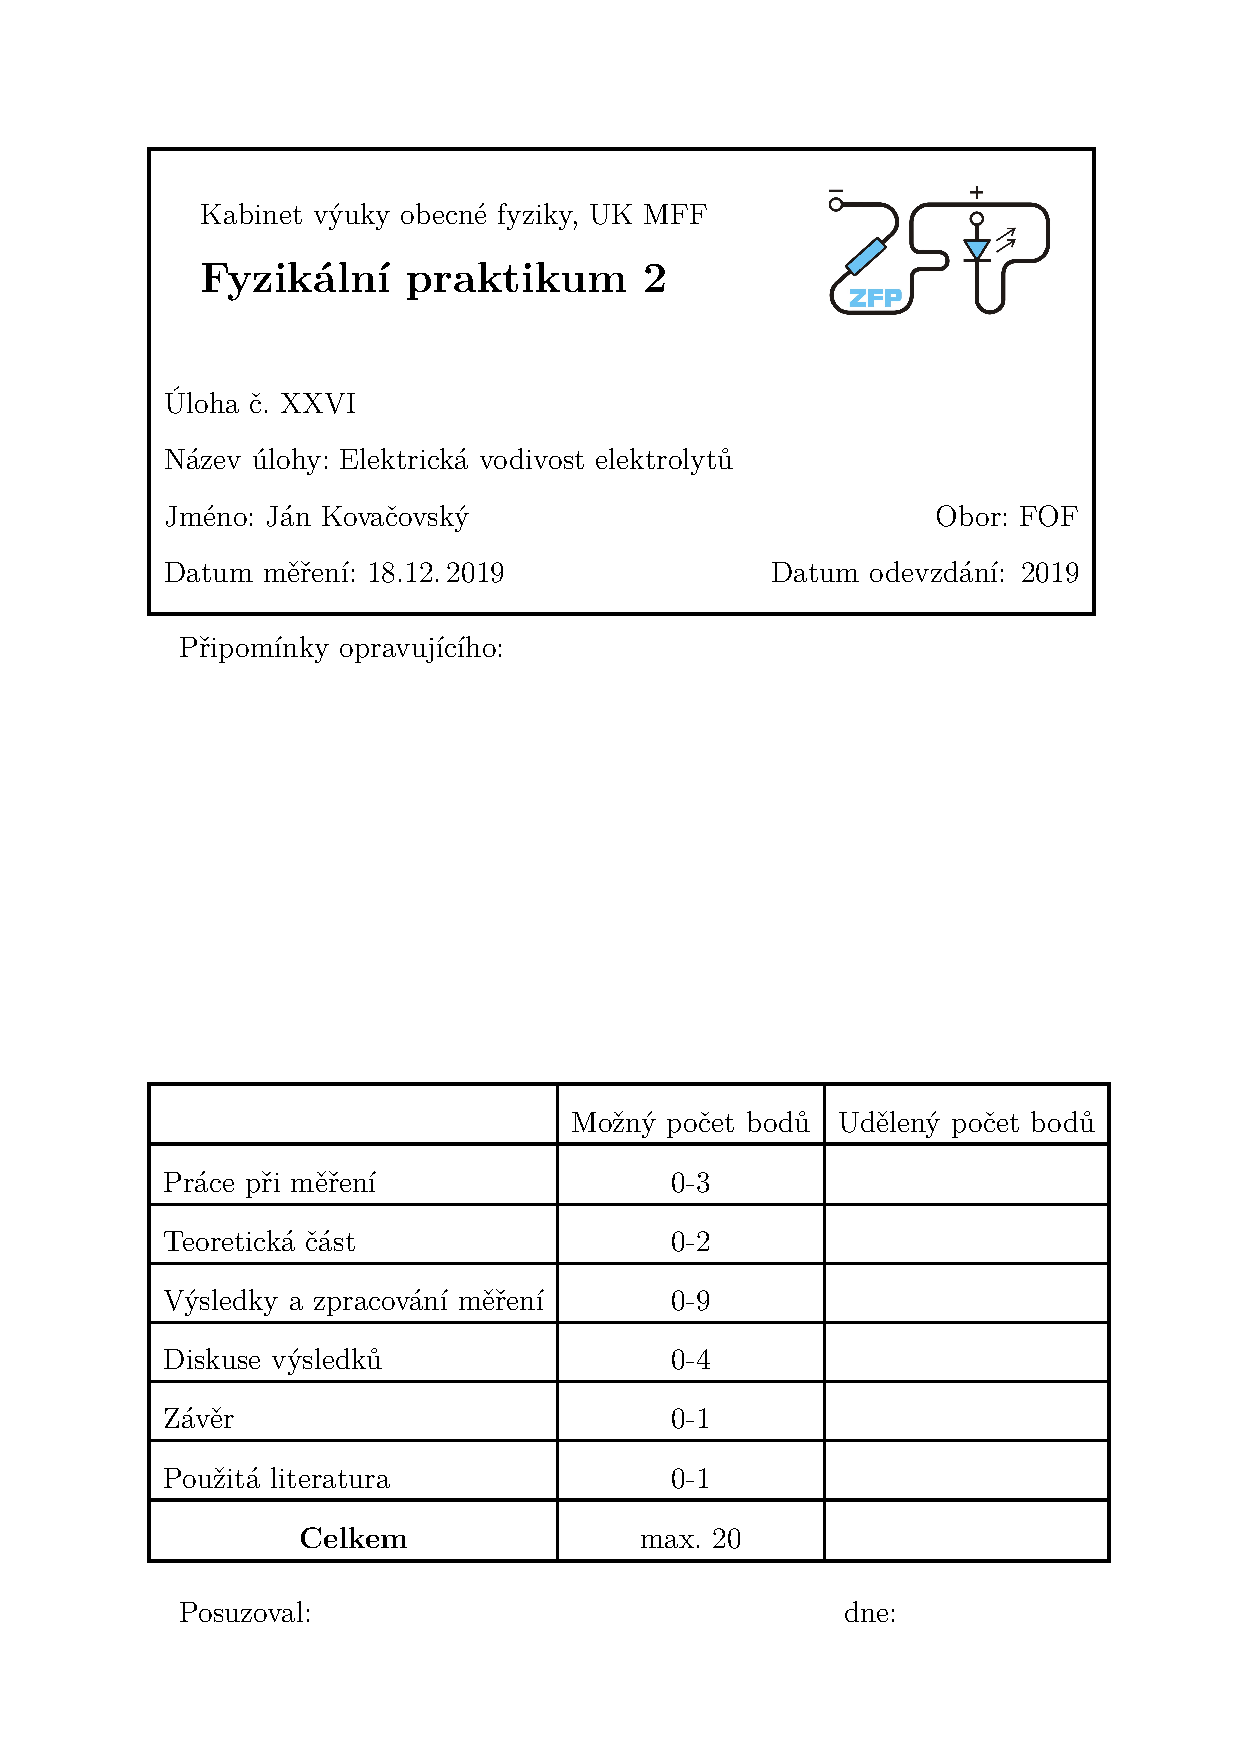
\includepdf[pages = 1]{titulka.pdf}

\section{Pracovná úloha}
\begin{enumerate}
    \item Zmerajte mernú elektrickú vodivosť destilovanej vody.
    \item Do odmerných baniek 100 ml napipetujte postupne 1, 2, 4, 6, 8 a 10 ml slabého a silného elektrolytu a doplňte banky do 100 ml (spodný meniskus hladiny sa musí prekrývať s ryskou).
    \item Zmerajte vodivosť pripravených vzoriek, korigujte ju o vodivosť vody a znázornite graficky.
    \item Stanovte molárnu vodivosť týchto vzoriek a znázornite ju graficky ako funkciu $\sqrt{c}$.
    \item Diskutujte rozdiely medzi koncentračnou závislosťou vodivosti a molárnou vodivosťou slabého a silného elektrolytu.
    \item Pre silný elektrolyt stanovte lineárnu extrapoláciu pre nekonečné zriedenie (nulovú koncentráciu) $\Lambda_0$.
\end{enumerate}

\section{Teória}
V elektrolytoch vznikajú disociáciou dva typy nábojov, kladné katióny a záporné anióny so všeobecne odlišným nábojom podľa pôvodne zlúčeniny, z ktorej vznikli. Vznik týchto iónov môžeme vyjadriť vzťahom podľa \cite{prak} 

\begin{equation}
    {K_x}{A_y} \leftrightarrow x{K^{y^+}} + y{A^{x^-}},
\end{equation}

kde pôvodná molekula obsahuje $x$ kladných katiónov $K$ s nábojom $y^+$ a $y$ záporných aniónov $A$ s nábojom $x^-$. Obecne je náboj $q$ nesený iónom daný celočíselným násobkom elementárneho náboja, čo môžeme vyjadriť vzťahom \cite{prak}

\begin{equation}
    q = {\pm}z{\cdot}e,
\end{equation}
kde $z$ je nábojové číslo iónu a $e$ = -1.602{$\cdot$}$10^{-19}$ C je podľa \cite{wiki} elementárny náboj. Kvôli veľkému počtu nosičov náboja však zavádzame tzv. Faradajovu konštantu \cite{prak}

\begin{equation}
    F = e{\cdot}N_A,
\end{equation}
kde $N_A$ je Avogadrova konštanta, číselne podľa \cite{avo} $N_A$ $\approx$ 6.022$\cdot$$10^{23}$ mol$^{-1}$.

Molekuly rozpustenej látky sú v elektrolyte disociované len čiastočne a preto zavádzame stupeň disociácie $\alpha$, ktorým vyjadrujeme ich mieru disociácie. Stupeň disociácie je definovaný podľa \cite{prak} ako podiel počtu disociovaných molekúl $n_{dis}$ k ich celkovému počtu $n$

\begin{equation}
    \alpha = \frac{n_{dis}}{n}.
\end{equation}

Elektrická vodivosť $\sigma$, definovaná ako schopnosť látky viesť elektrický prúd, je podľa \cite{prak} 

\begin{equation} \label{}
    i = \sigma{\cdot}E,    
\end{equation}
kde $i$ predstavuje prúdovú hustotu a $E$ intenzitu elektrického poľa. Pre elektrolyty platí obdobný vzťah \cite{prak}

\begin{equation}
    i = n_{dis}{\cdot}q{\cdot}v_D = \alpha{\cdot}c_M{\cdot}N_A{\cdot}z{\cdot}e{\cdot}v_D = \alpha{\cdot}c_M{\cdot}F{\cdot}z{\cdot}v_D,
\end{equation}
kde $v_D$ je stredná rýchlosť iónov a $c_M$ je ich molárna koncentrácia daná vzťahom podľa \cite{prak}

\begin{equation}
    c_M = \frac{n_i}{V},
\end{equation}
kde $n_i$ je počet molov i-tej rozpustenej látky a $V$ je celkový objem roztoku.

Aby platil Ohmov zákon, musí byť $v_D$ priamo úmerné $E$, preto \cite{prak}

\begin{equation}
    v_D = \mu{\cdot}E,
\end{equation}

kde konštanta úmernosti $\mu$ je tzv. pohyblivosť.

Pre elektrickú vodivosť $\sigma$ teda platí \cite{prak}

\begin{equation}
    \sigma = \alpha{\cdot}z{\cdot}e{\cdot}c_M{\cdot}N_A{\cdot}\mu = \alpha{\cdot}z{\cdot}F{\cdot}c_M{\cdot}{\mu}.
\end{equation}

\subsection{Silné elektrolyty}
Silné elektrolyty sú charakterizované stupňom disociácie rovným takmer jednej. Konduktivita teda rastie lineárne s molárnou koncentráciou. Definujeme preto molárnu vodivosť ako \cite{prak}

\begin{equation}
    \Lambda = \frac{\sigma}{c_M} = \alpha{\cdot}z{\cdot}e{\cdot}N_A{\cdot}\mu = \alpha{\cdot}z{\cdot}F{\cdot}\mu,
\end{equation}
kde molárna konduktivita $\Lambda$ je daná súčtom molárnej vodivosti katiónov a aniónov podľa \cite{prak} ako

\begin{equation}
    \Lambda = {\Lambda}_K + {\Lambda}_A = F(z_K{\cdot}{\mu}K + z_A{\cdot}{\mu}A).
\end{equation}

Koncentračná závislosť molárnej vodivosti je obecne rôzna pre silné a slabé elektrolyty. Pre silné elektrolyty platí empirický vzťah \cite{prak}

\begin{equation} \label{eq:zried}
    \Lambda = {\Lambda}^0 - k{\cdot}\sqrt{c_M},
\end{equation}
kde ${\Lambda}^0$ je limitná molárna konduktivita pri nekonečnom zriedení\footnote{t.j. pri nulovej koncentrácii}.

\subsection{Slabé elektrolyty}
Slabé elektrolyty sú charakterizované nízkym stupňom disociácie, v praxi rádu až $10^{-5}$. Tento stupeň disociácie je daný disociačnou konštantou $K_D$, ktorá môžeme podľa Guldberg-Waagovho zákona vyjadriť ako \cite{prak}

\begin{equation} \label{eq:sl1}
	K_D = \frac{[K^+]{\cdot}[A^-]}{[KA]},
\end{equation} 
kde $[K^+]$, $[A^-]$ a $[KA]$ sú rovnovážne koncentrácie katiónov $K^+$, aniónov $A^-$ a nedisociovaných molekúl $KA$. S využitím stupňa disociácie $\alpha$ môžeme vzťah (\ref{eq:sl1}) prepísať na \cite{prak}

\begin{equation}
    K_D = \frac{\alpha{\cdot}c_M{\cdot}\alpha{\cdot}c_M}{(1-\alpha){\cdot}c_M} \approx {\alpha}^2{\cdot}c_M,
\end{equation}
kde druhá rovnosť je len približná a platí dostatočne presne pre stupeň disociácie, ktorý je výrazne menší ako 1.

Vyjadrením stupňa disociácie $\alpha$ z tejto rovnice získame jeho závislosť na molárnej koncentrácii $c_M$ ako 

\begin{equation}
	\alpha = \sqrt{\frac{K_D}{c_M}}.
\end{equation}

Pre slabé elektrolyty teda platí, že s rastúcou koncentráciou klesá stupeň disociácie molekúl a konduktivita rastie nelineárne. Molárna konduktivita pri slabých elektrolytoch výrazne klesá s rastúcou koncentráciou. Tento pokles je daný práve poklesom stupňa disociácie.

\subsection{Spracovanie merania}
Chyby merania počítame podľa \cite{stat} ako
    \begin{equation} \label{stat:1}
        \sigma_v = \sqrt{\sigma_{\text{stat}}^2 + \sigma_{\text{mer}}^2 }
    \end{equation}
    kde $\sigma_{\text{stat}}$ je štatistická chyba a $\sigma_{\text{mer}}$ je chyba meradla (polovica dieliku na stupnici) pri meraní veličiny $v$. 
    
Pri výpočte chýb odvodených veličín používame Gaussov vzorec podľa \cite{stat}
    \begin{equation} \label{stat:2}
            \sigma_f = \sqrt{\sum_{i=1}^{n}\left( \frac{\partial f}{\partial x_i}\right)^2 \sigma_{x_i}^2}.
    \end{equation}
kde $x_i$ sú namerané veličiny v jednotlivých meraniach $i$, $n$ je ich počet a $\sigma$ je ich rozptyl, dopočítame ostávajúce chyby.

Pri digitálnych prístrojoch počítame chybu spôsobom uvedeným v návode. 

Na pipetovanie sme používali digitálnu mikropipetu s presnosťou minimálne\footnote{V rozsahu, v ktorom sme mikropipetu používali, t.j. od 1 ml do 10 ml, mala presnosť od 0.7\% do 0.5\%.} 0.7\%. Ako konduktometer sme používali Mettler Toledo s presnosťou 0.5\% a odmernú banku s len jednou ryskou na úrovni 100 ml, presnosť ktorej uvažujeme ako 1\%. 



\section{Výsledky merania}
Teplota v miestnosti a teda aj roztokov bola (20.9 $\pm$ 0.3)$\degree$C. Najskôr sme zmerali elektrickú vodivosť destilovanej vody, ktorú sme neskôr používali na riedenie meraných roztokov HCl a CH$_3$COOH. Na meranie sme používali konduktometer Mettler Toledo a vždy sme počkali, kým sa hodnota na ňom ustáli. Mernú vodivosť destilovanej vody sme zmerali trikrát, pred meraním HCl sme namerali 1.37 $\mu$S cm$^{-1}$, pred meraním $\ce{CH$_3$COOH}$ 1.35 $\mu$S cm$^{-1}$ a na konci merania, t.j. po zmeraní CH$_3$COOH, sme namerali elektrickú vodivosť destilovanej vody ako 1.36 $\mu$S cm$^{-1}$. Mernú vodivosť destilovanej vody ${\sigma}_v$ sme tak určili ako 

$$\text{${\sigma}_v$ = (1.36 $\pm$ 0.01) $\mu$S cm$^{-1}$.}$$

\subsection{Silný elektrolyt}
Následne sme zmerali elektrickú vodivosť ${\sigma}_{HCl}$ elektrolytu $\ce{HCl}$ a to od najnižšej koncentrácie, aby sme predišli zbytočnej chybe, ktorá by inak vznikla znečistením banky. Odpovedajúce hodnoty molárnej koncentrácie $c_M$ a dopočítané hodnoty molárnej vodivosti ${\Lambda}_{HCl}$. Tieto hodnoty sú uvedené v tabuľke \ref{tab:HCl} a vynesené do grafu \ref{graf:HCl}, kde chyby jednotlivých veličín sú počítané podľa vyššie uvedeného postupu. Hodnoty v grafe \ref{graf:HCl} sú preložené lineárnou funkciou tvaru $f(c_M)$ = a${\cdot}c_M$, ktorá bola vypočítaná metódou najmenších štvorcov programom \texttt{GNUPlot}. 

\begin{table}[!htbp]
\captionof{table}{Nameraná závislosť vodivosti $\sigma$ HCl na molárnej koncentrácii $c_M$ a dopočítané hodnoty molárnej vodivosti pre HCl}
\centering
\label{tab:HCl}
\begin{tabular}{|c|c|c|c|c|c|}
\hline
$V$ [ml] & $c_M$ [mol m$^{-3}$] & ${\sigma}_{HCl}$ [ $\mu$S cm$^{-1}$] &  ${\sigma}_{{\sigma}_{HCl}}$   & ${\Lambda}_{HCl}$ [mS m$^2$ mol$^{-1}$] & ${\sigma}_{{\Lambda}_{HCl}}$    \\ \hline
1      & 0.1                  & 48.9                                 & 0.2 & 48.9                                    & 0.9 \\ \hline
2      & 0.2                  & 97.5                                 & 0.5 & 48.8                                    & 0.9 \\ \hline
4      & 0.4                  & 196.2                                & 1.0 & 49.1                                    & 0.9 \\ \hline
6      & 0.6                  & 294.0                                & 1.5 & 49.0                                    & 0.9 \\ \hline
8      & 0.8                  & 392.0                                & 2.0 & 49.0                                    & 0.9 \\ \hline
10     & 1.0                  & 470.0                                & 2.4 & 47.0                                    & 1.3 \\ \hline
\end{tabular}
\end{table}

Hodnotu molárnej vodivosti pri nekonečnom zriedení $\Lambda^0$ sme určili lineárnou extrapoláciou hodnôt v grafe \ref{graf:LHCl}. Zo vzťahu (\ref{eq:zried}) teda dostávame $\Lambda^0$ = (49 $\pm$ 1) mS${\cdot}$m$^2$${\cdot}$mol$^{-1}$, kde chyba je určená chybou fitu.

\newpage
Chybu vypočítanej molárnej vodivosti $\Lambda$, sme vypočítali podľa (\ref{stat:2}) ako 

\begin{equation} \label{eq:stat:Lambda}
    \sigma_{\Lambda} = {\Lambda}\sqrt{\left(\frac{{\sigma}_{\sigma}}{\sigma}\right)^2 + \left(\frac{{\sigma}_{V_{100}}}{V_{100}}\right)^2 + \left(\frac{{\sigma}_{V}}{V}\right)^2}, 
\end{equation}
kde $V$ je objem elektrolytu vo vode a $V_{100}$ je celkový objem.
 
\begin{graph}[H]
		\centering
		% GNUPLOT: LaTeX picture with Postscript
\begingroup
  \makeatletter
  \providecommand\color[2][]{%
    \GenericError{(gnuplot) \space\space\space\@spaces}{%
      Package color not loaded in conjunction with
      terminal option `colourtext'%
    }{See the gnuplot documentation for explanation.%
    }{Either use 'blacktext' in gnuplot or load the package
      color.sty in LaTeX.}%
    \renewcommand\color[2][]{}%
  }%
  \providecommand\includegraphics[2][]{%
    \GenericError{(gnuplot) \space\space\space\@spaces}{%
      Package graphicx or graphics not loaded%
    }{See the gnuplot documentation for explanation.%
    }{The gnuplot epslatex terminal needs graphicx.sty or graphics.sty.}%
    \renewcommand\includegraphics[2][]{}%
  }%
  \providecommand\rotatebox[2]{#2}%
  \@ifundefined{ifGPcolor}{%
    \newif\ifGPcolor
    \GPcolorfalse
  }{}%
  \@ifundefined{ifGPblacktext}{%
    \newif\ifGPblacktext
    \GPblacktexttrue
  }{}%
  % define a \g@addto@macro without @ in the name:
  \let\gplgaddtomacro\g@addto@macro
  % define empty templates for all commands taking text:
  \gdef\gplbacktext{}%
  \gdef\gplfronttext{}%
  \makeatother
  \ifGPblacktext
    % no textcolor at all
    \def\colorrgb#1{}%
    \def\colorgray#1{}%
  \else
    % gray or color?
    \ifGPcolor
      \def\colorrgb#1{\color[rgb]{#1}}%
      \def\colorgray#1{\color[gray]{#1}}%
      \expandafter\def\csname LTw\endcsname{\color{white}}%
      \expandafter\def\csname LTb\endcsname{\color{black}}%
      \expandafter\def\csname LTa\endcsname{\color{black}}%
      \expandafter\def\csname LT0\endcsname{\color[rgb]{1,0,0}}%
      \expandafter\def\csname LT1\endcsname{\color[rgb]{0,1,0}}%
      \expandafter\def\csname LT2\endcsname{\color[rgb]{0,0,1}}%
      \expandafter\def\csname LT3\endcsname{\color[rgb]{1,0,1}}%
      \expandafter\def\csname LT4\endcsname{\color[rgb]{0,1,1}}%
      \expandafter\def\csname LT5\endcsname{\color[rgb]{1,1,0}}%
      \expandafter\def\csname LT6\endcsname{\color[rgb]{0,0,0}}%
      \expandafter\def\csname LT7\endcsname{\color[rgb]{1,0.3,0}}%
      \expandafter\def\csname LT8\endcsname{\color[rgb]{0.5,0.5,0.5}}%
    \else
      % gray
      \def\colorrgb#1{\color{black}}%
      \def\colorgray#1{\color[gray]{#1}}%
      \expandafter\def\csname LTw\endcsname{\color{white}}%
      \expandafter\def\csname LTb\endcsname{\color{black}}%
      \expandafter\def\csname LTa\endcsname{\color{black}}%
      \expandafter\def\csname LT0\endcsname{\color{black}}%
      \expandafter\def\csname LT1\endcsname{\color{black}}%
      \expandafter\def\csname LT2\endcsname{\color{black}}%
      \expandafter\def\csname LT3\endcsname{\color{black}}%
      \expandafter\def\csname LT4\endcsname{\color{black}}%
      \expandafter\def\csname LT5\endcsname{\color{black}}%
      \expandafter\def\csname LT6\endcsname{\color{black}}%
      \expandafter\def\csname LT7\endcsname{\color{black}}%
      \expandafter\def\csname LT8\endcsname{\color{black}}%
    \fi
  \fi
    \setlength{\unitlength}{0.0500bp}%
    \ifx\gptboxheight\undefined%
      \newlength{\gptboxheight}%
      \newlength{\gptboxwidth}%
      \newsavebox{\gptboxtext}%
    \fi%
    \setlength{\fboxrule}{0.5pt}%
    \setlength{\fboxsep}{1pt}%
\begin{picture}(7370.00,4534.00)%
    \gplgaddtomacro\gplbacktext{%
      \csname LTb\endcsname%%
      \put(814,704){\makebox(0,0)[r]{\strut{}$0$}}%
      \csname LTb\endcsname%%
      \put(814,1426){\makebox(0,0)[r]{\strut{}$100$}}%
      \csname LTb\endcsname%%
      \put(814,2148){\makebox(0,0)[r]{\strut{}$200$}}%
      \csname LTb\endcsname%%
      \put(814,2869){\makebox(0,0)[r]{\strut{}$300$}}%
      \csname LTb\endcsname%%
      \put(814,3591){\makebox(0,0)[r]{\strut{}$400$}}%
      \csname LTb\endcsname%%
      \put(814,4313){\makebox(0,0)[r]{\strut{}$500$}}%
      \csname LTb\endcsname%%
      \put(946,484){\makebox(0,0){\strut{}$0$}}%
      \csname LTb\endcsname%%
      \put(2094,484){\makebox(0,0){\strut{}$0.2$}}%
      \csname LTb\endcsname%%
      \put(3242,484){\makebox(0,0){\strut{}$0.4$}}%
      \csname LTb\endcsname%%
      \put(4390,484){\makebox(0,0){\strut{}$0.6$}}%
      \csname LTb\endcsname%%
      \put(5538,484){\makebox(0,0){\strut{}$0.8$}}%
      \csname LTb\endcsname%%
      \put(6686,484){\makebox(0,0){\strut{}$1$}}%
    }%
    \gplgaddtomacro\gplfronttext{%
      \csname LTb\endcsname%%
      \put(198,2508){\rotatebox{-270}{\makebox(0,0){\strut{}$\sigma$ [${\mu}$S/cm]}}}%
      \put(3959,154){\makebox(0,0){\strut{}$c_M$ [mMol/L]}}%
      \csname LTb\endcsname%%
      \put(5986,1097){\makebox(0,0)[r]{\strut{}$f$($c_M$) = 480.9$c_M$}}%
      \csname LTb\endcsname%%
      \put(5986,877){\makebox(0,0)[r]{\strut{}namerané hodnoty}}%
    }%
    \gplbacktext
    \put(0,0){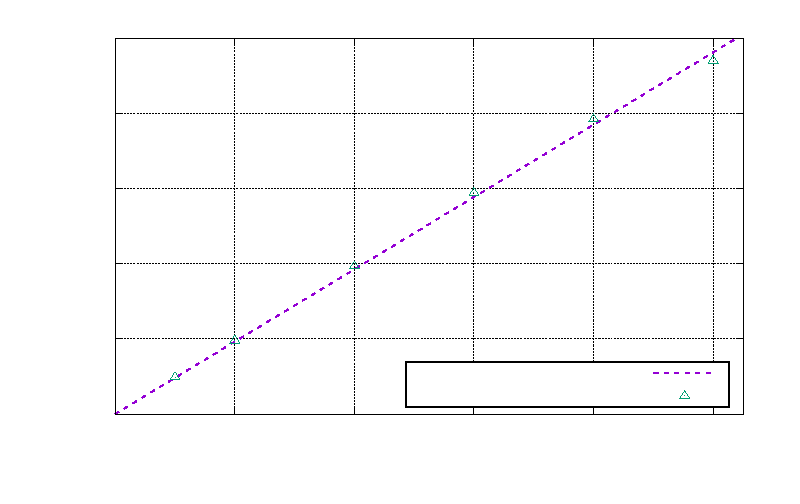
\includegraphics{HCl}}%
    \gplfronttext
  \end{picture}%
\endgroup

		\caption{Závislosť vodivosti $\sigma$ HCl na molárnej koncentrácii $c_M$}
		\label{graf:HCl}
\end{graph}

Parameter $a$ fitovanej funkcie vypočítaný programom \texttt{GNUPlot} vyšiel ako $a$ = (480.9 $\pm$ 4.4).

\begin{graph}[H]
		\centering
		% GNUPLOT: LaTeX picture with Postscript
\begingroup
  \makeatletter
  \providecommand\color[2][]{%
    \GenericError{(gnuplot) \space\space\space\@spaces}{%
      Package color not loaded in conjunction with
      terminal option `colourtext'%
    }{See the gnuplot documentation for explanation.%
    }{Either use 'blacktext' in gnuplot or load the package
      color.sty in LaTeX.}%
    \renewcommand\color[2][]{}%
  }%
  \providecommand\includegraphics[2][]{%
    \GenericError{(gnuplot) \space\space\space\@spaces}{%
      Package graphicx or graphics not loaded%
    }{See the gnuplot documentation for explanation.%
    }{The gnuplot epslatex terminal needs graphicx.sty or graphics.sty.}%
    \renewcommand\includegraphics[2][]{}%
  }%
  \providecommand\rotatebox[2]{#2}%
  \@ifundefined{ifGPcolor}{%
    \newif\ifGPcolor
    \GPcolorfalse
  }{}%
  \@ifundefined{ifGPblacktext}{%
    \newif\ifGPblacktext
    \GPblacktexttrue
  }{}%
  % define a \g@addto@macro without @ in the name:
  \let\gplgaddtomacro\g@addto@macro
  % define empty templates for all commands taking text:
  \gdef\gplbacktext{}%
  \gdef\gplfronttext{}%
  \makeatother
  \ifGPblacktext
    % no textcolor at all
    \def\colorrgb#1{}%
    \def\colorgray#1{}%
  \else
    % gray or color?
    \ifGPcolor
      \def\colorrgb#1{\color[rgb]{#1}}%
      \def\colorgray#1{\color[gray]{#1}}%
      \expandafter\def\csname LTw\endcsname{\color{white}}%
      \expandafter\def\csname LTb\endcsname{\color{black}}%
      \expandafter\def\csname LTa\endcsname{\color{black}}%
      \expandafter\def\csname LT0\endcsname{\color[rgb]{1,0,0}}%
      \expandafter\def\csname LT1\endcsname{\color[rgb]{0,1,0}}%
      \expandafter\def\csname LT2\endcsname{\color[rgb]{0,0,1}}%
      \expandafter\def\csname LT3\endcsname{\color[rgb]{1,0,1}}%
      \expandafter\def\csname LT4\endcsname{\color[rgb]{0,1,1}}%
      \expandafter\def\csname LT5\endcsname{\color[rgb]{1,1,0}}%
      \expandafter\def\csname LT6\endcsname{\color[rgb]{0,0,0}}%
      \expandafter\def\csname LT7\endcsname{\color[rgb]{1,0.3,0}}%
      \expandafter\def\csname LT8\endcsname{\color[rgb]{0.5,0.5,0.5}}%
    \else
      % gray
      \def\colorrgb#1{\color{black}}%
      \def\colorgray#1{\color[gray]{#1}}%
      \expandafter\def\csname LTw\endcsname{\color{white}}%
      \expandafter\def\csname LTb\endcsname{\color{black}}%
      \expandafter\def\csname LTa\endcsname{\color{black}}%
      \expandafter\def\csname LT0\endcsname{\color{black}}%
      \expandafter\def\csname LT1\endcsname{\color{black}}%
      \expandafter\def\csname LT2\endcsname{\color{black}}%
      \expandafter\def\csname LT3\endcsname{\color{black}}%
      \expandafter\def\csname LT4\endcsname{\color{black}}%
      \expandafter\def\csname LT5\endcsname{\color{black}}%
      \expandafter\def\csname LT6\endcsname{\color{black}}%
      \expandafter\def\csname LT7\endcsname{\color{black}}%
      \expandafter\def\csname LT8\endcsname{\color{black}}%
    \fi
  \fi
    \setlength{\unitlength}{0.0500bp}%
    \ifx\gptboxheight\undefined%
      \newlength{\gptboxheight}%
      \newlength{\gptboxwidth}%
      \newsavebox{\gptboxtext}%
    \fi%
    \setlength{\fboxrule}{0.5pt}%
    \setlength{\fboxsep}{1pt}%
\begin{picture}(7370.00,4534.00)%
    \gplgaddtomacro\gplbacktext{%
      \csname LTb\endcsname%%
      \put(946,704){\makebox(0,0)[r]{\strut{}$46.5$}}%
      \csname LTb\endcsname%%
      \put(946,1220){\makebox(0,0)[r]{\strut{}$47$}}%
      \csname LTb\endcsname%%
      \put(946,1735){\makebox(0,0)[r]{\strut{}$47.5$}}%
      \csname LTb\endcsname%%
      \put(946,2251){\makebox(0,0)[r]{\strut{}$48$}}%
      \csname LTb\endcsname%%
      \put(946,2766){\makebox(0,0)[r]{\strut{}$48.5$}}%
      \csname LTb\endcsname%%
      \put(946,3282){\makebox(0,0)[r]{\strut{}$49$}}%
      \csname LTb\endcsname%%
      \put(946,3797){\makebox(0,0)[r]{\strut{}$49.5$}}%
      \csname LTb\endcsname%%
      \put(946,4313){\makebox(0,0)[r]{\strut{}$50$}}%
      \csname LTb\endcsname%%
      \put(1078,484){\makebox(0,0){\strut{}$0$}}%
      \csname LTb\endcsname%%
      \put(2201,484){\makebox(0,0){\strut{}$0.2$}}%
      \csname LTb\endcsname%%
      \put(3324,484){\makebox(0,0){\strut{}$0.4$}}%
      \csname LTb\endcsname%%
      \put(4447,484){\makebox(0,0){\strut{}$0.6$}}%
      \csname LTb\endcsname%%
      \put(5569,484){\makebox(0,0){\strut{}$0.8$}}%
      \csname LTb\endcsname%%
      \put(6692,484){\makebox(0,0){\strut{}$1$}}%
    }%
    \gplgaddtomacro\gplfronttext{%
      \csname LTb\endcsname%%
      \put(198,2508){\rotatebox{-270}{\makebox(0,0){\strut{}$\Lambda$ [mS m$^2$ mol$^{-1}$] }}}%
      \put(4025,154){\makebox(0,0){\strut{}$\sqrt{c_M}$ [$(\text{mol m$^{-3}$})^{1/2}$]}}%
      \csname LTb\endcsname%%
      \put(4114,1537){\makebox(0,0)[r]{\strut{}$f(x) = 0.29x$ + 48.78}}%
      \csname LTb\endcsname%%
      \put(4114,1317){\makebox(0,0)[r]{\strut{}$g(x) = 48.96$}}%
      \csname LTb\endcsname%%
      \put(4114,1097){\makebox(0,0)[r]{\strut{}Molárna vodivosť HCl}}%
      \csname LTb\endcsname%%
      \put(4114,877){\makebox(0,0)[r]{\strut{}Anomálna hodnota}}%
    }%
    \gplbacktext
    \put(0,0){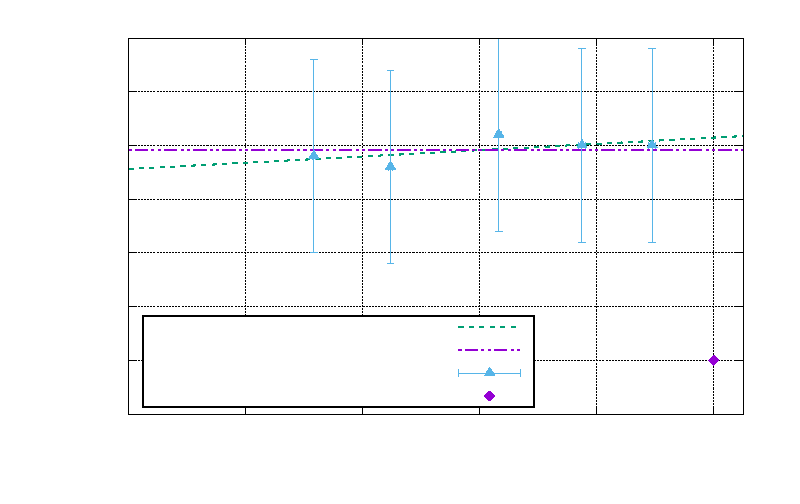
\includegraphics{LHCl}}%
    \gplfronttext
  \end{picture}%
\endgroup

		\caption{Závislosť molárnej vodivosti $\Lambda$ HCl na druhej odmocnine z molárnej koncentrácie $c_M$}
		\label{graf:LHCl}
\end{graph}


\subsection{Slabé elektrolyty}
Postup práce bol analogický predošlej úlohe so silným elektrolytom. Meranie sme si obohatili o pár hodnôt aby sme boli schopní určiť jednotlivé závislosti presnejšie. Namerané hodnoty elektrickej vodivosti, a objemu, resp. koncentrácii roztokov spolu s vypočítanými hodnotami molárnej vodivosti $\Lambda_{CH_3}$ sú uvedené v tab. \ref{tab:CH3}. Chyby tohoto merania boli vypočítané vyššie uvedeným postupom a chyba $\Lambda_{CH_3}$ vzťahom (\ref{eq:stat:Lambda}). 

\begin{table}[H]
\centering
\captionof{table}{Nameraná závislosť vodivosti $\sigma$ CH$_3$COOH na molárnej koncentrácii $c_M$ a dopočítané hodnoty molárnej vodivosti pre CH$_3$COOH} 
\label{tab:CH3}
\begin{tabular}{|c|c|c|c|c|c|} 
\hline
$V$ [ml] & $c_M$ [mol m$^{-3}$] & ${\sigma}_{CH_3}$ [ $\mu$S cm$^{-1}$] &  ${\sigma}_{{\sigma}_{CH_3}}$   & ${\Lambda}_{CH_3}$ [mS m$^2$ mol$^{-1}$] &${\sigma}_{{\Lambda}_{CH_3}}$     \\ \hline
1      & 0.5                  & 33.2                                 & 0.2 & 33.2                                    & 0.2 \\ \hline
2      & 1.0                  & 47.8                                 & 0.2 & 23.9                                    & 0.2 \\ \hline
3      & 1.5                  & 58.5                                 & 0.3 & 19.5                                    & 0.1 \\ \hline
6      & 3.0                  & 84.9                                 & 0.4 & 14.2                                    & 0.1 \\ \hline
8      & 4.0                  & 98.2                                 & 0.5 & 12.3                                    & 0.1 \\ \hline
10     & 5.0                    & 108.9                                & 0.5 & 10.9                                    & 0.1 \\ \hline
1.5    & 0.8                 & 39.5                                 & 0.2 & 26.3                                    & 0.2 \\ \hline
4      & 2.0                  & 66.3                                 & 0.3 & 16.6                                    & 0.1 \\ \hline
\end{tabular}
\end{table}

Hodnoty elektrickej vodivosti $\sigma$ v závislosti na molárnej koncentrácii $c_M$ boli vynesené do grafu \ref{graf:CH3}, kde boli preložené mocninou funkciou tvaru $f(c_M) = a{\cdot}\sqrt{c_M}$. 

\begin{graph}[H]
		\centering
		% GNUPLOT: LaTeX picture with Postscript
\begingroup
  \makeatletter
  \providecommand\color[2][]{%
    \GenericError{(gnuplot) \space\space\space\@spaces}{%
      Package color not loaded in conjunction with
      terminal option `colourtext'%
    }{See the gnuplot documentation for explanation.%
    }{Either use 'blacktext' in gnuplot or load the package
      color.sty in LaTeX.}%
    \renewcommand\color[2][]{}%
  }%
  \providecommand\includegraphics[2][]{%
    \GenericError{(gnuplot) \space\space\space\@spaces}{%
      Package graphicx or graphics not loaded%
    }{See the gnuplot documentation for explanation.%
    }{The gnuplot epslatex terminal needs graphicx.sty or graphics.sty.}%
    \renewcommand\includegraphics[2][]{}%
  }%
  \providecommand\rotatebox[2]{#2}%
  \@ifundefined{ifGPcolor}{%
    \newif\ifGPcolor
    \GPcolorfalse
  }{}%
  \@ifundefined{ifGPblacktext}{%
    \newif\ifGPblacktext
    \GPblacktexttrue
  }{}%
  % define a \g@addto@macro without @ in the name:
  \let\gplgaddtomacro\g@addto@macro
  % define empty templates for all commands taking text:
  \gdef\gplbacktext{}%
  \gdef\gplfronttext{}%
  \makeatother
  \ifGPblacktext
    % no textcolor at all
    \def\colorrgb#1{}%
    \def\colorgray#1{}%
  \else
    % gray or color?
    \ifGPcolor
      \def\colorrgb#1{\color[rgb]{#1}}%
      \def\colorgray#1{\color[gray]{#1}}%
      \expandafter\def\csname LTw\endcsname{\color{white}}%
      \expandafter\def\csname LTb\endcsname{\color{black}}%
      \expandafter\def\csname LTa\endcsname{\color{black}}%
      \expandafter\def\csname LT0\endcsname{\color[rgb]{1,0,0}}%
      \expandafter\def\csname LT1\endcsname{\color[rgb]{0,1,0}}%
      \expandafter\def\csname LT2\endcsname{\color[rgb]{0,0,1}}%
      \expandafter\def\csname LT3\endcsname{\color[rgb]{1,0,1}}%
      \expandafter\def\csname LT4\endcsname{\color[rgb]{0,1,1}}%
      \expandafter\def\csname LT5\endcsname{\color[rgb]{1,1,0}}%
      \expandafter\def\csname LT6\endcsname{\color[rgb]{0,0,0}}%
      \expandafter\def\csname LT7\endcsname{\color[rgb]{1,0.3,0}}%
      \expandafter\def\csname LT8\endcsname{\color[rgb]{0.5,0.5,0.5}}%
    \else
      % gray
      \def\colorrgb#1{\color{black}}%
      \def\colorgray#1{\color[gray]{#1}}%
      \expandafter\def\csname LTw\endcsname{\color{white}}%
      \expandafter\def\csname LTb\endcsname{\color{black}}%
      \expandafter\def\csname LTa\endcsname{\color{black}}%
      \expandafter\def\csname LT0\endcsname{\color{black}}%
      \expandafter\def\csname LT1\endcsname{\color{black}}%
      \expandafter\def\csname LT2\endcsname{\color{black}}%
      \expandafter\def\csname LT3\endcsname{\color{black}}%
      \expandafter\def\csname LT4\endcsname{\color{black}}%
      \expandafter\def\csname LT5\endcsname{\color{black}}%
      \expandafter\def\csname LT6\endcsname{\color{black}}%
      \expandafter\def\csname LT7\endcsname{\color{black}}%
      \expandafter\def\csname LT8\endcsname{\color{black}}%
    \fi
  \fi
    \setlength{\unitlength}{0.0500bp}%
    \ifx\gptboxheight\undefined%
      \newlength{\gptboxheight}%
      \newlength{\gptboxwidth}%
      \newsavebox{\gptboxtext}%
    \fi%
    \setlength{\fboxrule}{0.5pt}%
    \setlength{\fboxsep}{1pt}%
\begin{picture}(8502.00,4534.00)%
    \gplgaddtomacro\gplbacktext{%
      \csname LTb\endcsname%%
      \put(814,704){\makebox(0,0)[r]{\strut{}$0$}}%
      \csname LTb\endcsname%%
      \put(814,1348){\makebox(0,0)[r]{\strut{}$20$}}%
      \csname LTb\endcsname%%
      \put(814,1993){\makebox(0,0)[r]{\strut{}$40$}}%
      \csname LTb\endcsname%%
      \put(814,2637){\makebox(0,0)[r]{\strut{}$60$}}%
      \csname LTb\endcsname%%
      \put(814,3282){\makebox(0,0)[r]{\strut{}$80$}}%
      \csname LTb\endcsname%%
      \put(814,3926){\makebox(0,0)[r]{\strut{}$100$}}%
      \csname LTb\endcsname%%
      \put(946,484){\makebox(0,0){\strut{}$0$}}%
      \csname LTb\endcsname%%
      \put(2310,484){\makebox(0,0){\strut{}$1.0$}}%
      \csname LTb\endcsname%%
      \put(3673,484){\makebox(0,0){\strut{}$2.0$}}%
      \csname LTb\endcsname%%
      \put(5037,484){\makebox(0,0){\strut{}$3.0$}}%
      \csname LTb\endcsname%%
      \put(6400,484){\makebox(0,0){\strut{}$4.0$}}%
      \csname LTb\endcsname%%
      \put(7764,484){\makebox(0,0){\strut{}$5.0$}}%
    }%
    \gplgaddtomacro\gplfronttext{%
      \csname LTb\endcsname%%
      \put(198,2508){\rotatebox{-270}{\makebox(0,0){\strut{}$\sigma$ [$\mu$S/cm]}}}%
      \put(4525,154){\makebox(0,0){\strut{}$c_M$ [mMol/L]}}%
      \csname LTb\endcsname%%
      \put(7118,1097){\makebox(0,0)[r]{\strut{}$f(c_M)$ = 108.07${\cdot}\sqrt{c_M}$}}%
      \csname LTb\endcsname%%
      \put(7118,877){\makebox(0,0)[r]{\strut{}namerané hodnoty}}%
    }%
    \gplbacktext
    \put(0,0){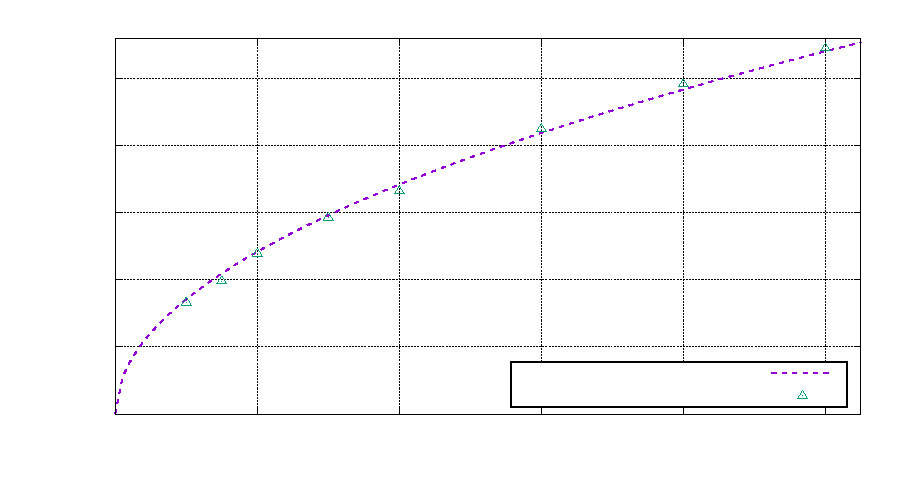
\includegraphics{CH3}}%
    \gplfronttext
  \end{picture}%
\endgroup

		\caption{Závislosť vodivosti $\sigma$ CH$_3$COOH na molárnej koncentrácii $c_M$}
		\label{graf:CH3}
\end{graph} 

\begin{graph}[H]
		\centering
		% GNUPLOT: LaTeX picture with Postscript
\begingroup
  \makeatletter
  \providecommand\color[2][]{%
    \GenericError{(gnuplot) \space\space\space\@spaces}{%
      Package color not loaded in conjunction with
      terminal option `colourtext'%
    }{See the gnuplot documentation for explanation.%
    }{Either use 'blacktext' in gnuplot or load the package
      color.sty in LaTeX.}%
    \renewcommand\color[2][]{}%
  }%
  \providecommand\includegraphics[2][]{%
    \GenericError{(gnuplot) \space\space\space\@spaces}{%
      Package graphicx or graphics not loaded%
    }{See the gnuplot documentation for explanation.%
    }{The gnuplot epslatex terminal needs graphicx.sty or graphics.sty.}%
    \renewcommand\includegraphics[2][]{}%
  }%
  \providecommand\rotatebox[2]{#2}%
  \@ifundefined{ifGPcolor}{%
    \newif\ifGPcolor
    \GPcolorfalse
  }{}%
  \@ifundefined{ifGPblacktext}{%
    \newif\ifGPblacktext
    \GPblacktexttrue
  }{}%
  % define a \g@addto@macro without @ in the name:
  \let\gplgaddtomacro\g@addto@macro
  % define empty templates for all commands taking text:
  \gdef\gplbacktext{}%
  \gdef\gplfronttext{}%
  \makeatother
  \ifGPblacktext
    % no textcolor at all
    \def\colorrgb#1{}%
    \def\colorgray#1{}%
  \else
    % gray or color?
    \ifGPcolor
      \def\colorrgb#1{\color[rgb]{#1}}%
      \def\colorgray#1{\color[gray]{#1}}%
      \expandafter\def\csname LTw\endcsname{\color{white}}%
      \expandafter\def\csname LTb\endcsname{\color{black}}%
      \expandafter\def\csname LTa\endcsname{\color{black}}%
      \expandafter\def\csname LT0\endcsname{\color[rgb]{1,0,0}}%
      \expandafter\def\csname LT1\endcsname{\color[rgb]{0,1,0}}%
      \expandafter\def\csname LT2\endcsname{\color[rgb]{0,0,1}}%
      \expandafter\def\csname LT3\endcsname{\color[rgb]{1,0,1}}%
      \expandafter\def\csname LT4\endcsname{\color[rgb]{0,1,1}}%
      \expandafter\def\csname LT5\endcsname{\color[rgb]{1,1,0}}%
      \expandafter\def\csname LT6\endcsname{\color[rgb]{0,0,0}}%
      \expandafter\def\csname LT7\endcsname{\color[rgb]{1,0.3,0}}%
      \expandafter\def\csname LT8\endcsname{\color[rgb]{0.5,0.5,0.5}}%
    \else
      % gray
      \def\colorrgb#1{\color{black}}%
      \def\colorgray#1{\color[gray]{#1}}%
      \expandafter\def\csname LTw\endcsname{\color{white}}%
      \expandafter\def\csname LTb\endcsname{\color{black}}%
      \expandafter\def\csname LTa\endcsname{\color{black}}%
      \expandafter\def\csname LT0\endcsname{\color{black}}%
      \expandafter\def\csname LT1\endcsname{\color{black}}%
      \expandafter\def\csname LT2\endcsname{\color{black}}%
      \expandafter\def\csname LT3\endcsname{\color{black}}%
      \expandafter\def\csname LT4\endcsname{\color{black}}%
      \expandafter\def\csname LT5\endcsname{\color{black}}%
      \expandafter\def\csname LT6\endcsname{\color{black}}%
      \expandafter\def\csname LT7\endcsname{\color{black}}%
      \expandafter\def\csname LT8\endcsname{\color{black}}%
    \fi
  \fi
    \setlength{\unitlength}{0.0500bp}%
    \ifx\gptboxheight\undefined%
      \newlength{\gptboxheight}%
      \newlength{\gptboxwidth}%
      \newsavebox{\gptboxtext}%
    \fi%
    \setlength{\fboxrule}{0.5pt}%
    \setlength{\fboxsep}{1pt}%
\begin{picture}(9070.00,4534.00)%
    \gplgaddtomacro\gplbacktext{%
      \csname LTb\endcsname%%
      \put(682,704){\makebox(0,0)[r]{\strut{}$10$}}%
      \csname LTb\endcsname%%
      \put(682,1426){\makebox(0,0)[r]{\strut{}$15$}}%
      \csname LTb\endcsname%%
      \put(682,2148){\makebox(0,0)[r]{\strut{}$20$}}%
      \csname LTb\endcsname%%
      \put(682,2869){\makebox(0,0)[r]{\strut{}$25$}}%
      \csname LTb\endcsname%%
      \put(682,3591){\makebox(0,0)[r]{\strut{}$30$}}%
      \csname LTb\endcsname%%
      \put(682,4313){\makebox(0,0)[r]{\strut{}$35$}}%
      \csname LTb\endcsname%%
      \put(814,484){\makebox(0,0){\strut{}$0.6$}}%
      \csname LTb\endcsname%%
      \put(1687,484){\makebox(0,0){\strut{}$0.8$}}%
      \csname LTb\endcsname%%
      \put(2560,484){\makebox(0,0){\strut{}$1$}}%
      \csname LTb\endcsname%%
      \put(3434,484){\makebox(0,0){\strut{}$1.2$}}%
      \csname LTb\endcsname%%
      \put(4307,484){\makebox(0,0){\strut{}$1.4$}}%
      \csname LTb\endcsname%%
      \put(5180,484){\makebox(0,0){\strut{}$1.6$}}%
      \csname LTb\endcsname%%
      \put(6053,484){\makebox(0,0){\strut{}$1.8$}}%
      \csname LTb\endcsname%%
      \put(6927,484){\makebox(0,0){\strut{}$2$}}%
      \csname LTb\endcsname%%
      \put(7800,484){\makebox(0,0){\strut{}$2.2$}}%
      \csname LTb\endcsname%%
      \put(8673,484){\makebox(0,0){\strut{}$2.4$}}%
    }%
    \gplgaddtomacro\gplfronttext{%
      \csname LTb\endcsname%%
      \put(198,2508){\rotatebox{-270}{\makebox(0,0){\strut{}$\Lambda$ [mS m$^2$ mol$^{-1}$]}}}%
      \put(4743,154){\makebox(0,0){\strut{}$\sqrt{c_M}$ [$(\text{mol m$^{-3}$})^{1/2}$}}%
      \csname LTb\endcsname%%
      \put(7686,4140){\makebox(0,0)[r]{\strut{}$f(x) = 23.57{\cdot}x^{-1}$}}%
      \csname LTb\endcsname%%
      \put(7686,3920){\makebox(0,0)[r]{\strut{}molárna vodivosť CH$_3$COOH}}%
    }%
    \gplbacktext
    \put(0,0){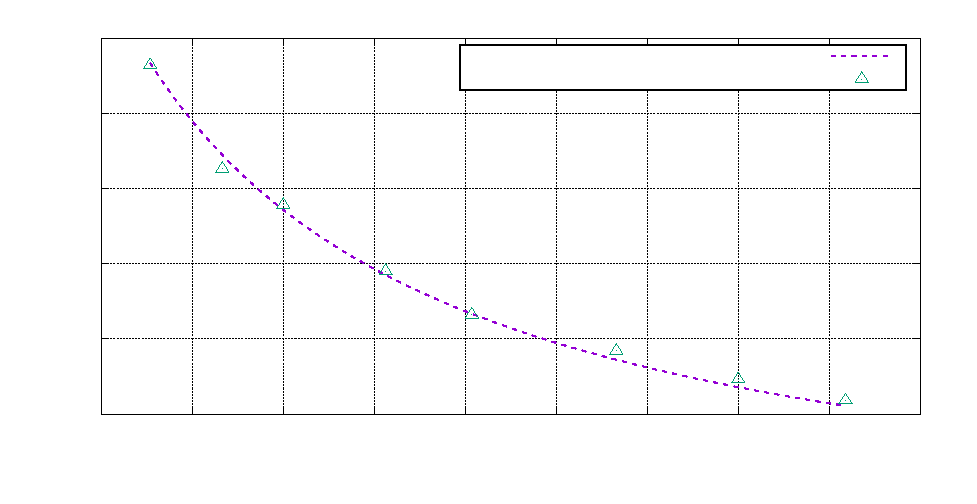
\includegraphics{CH3L}}%
    \gplfronttext
  \end{picture}%
\endgroup

		\caption{Závislosť molárnej vodivosti $\Lambda$ CH$_3$COOH na druhej odmocnine z molárnej koncentrácie $c_M$}
		\label{graf:CH3L}
\end{graph}

\section{Diskusia výsledkov}
Najskôr sme namerali vodivosť destilovanej vody, ktorú sme počas experimentu používali. Táto hodnota nás nejako veľmi neprekvapila a neuvažovali sme ňou možnú kontamináciu roztokov pri našich meraniach. V tejto destilovanej vode sa vyskytovali určité nečistoty ako aj OH$^-$ a H$^+$, ktoré sú taktiež schopné niesť náboj a nedá sa ich zbaviť. Na rozdiel od nedestilovanej vody, ktorej vodivosť bola vyššia ako vodivosť slabého elektrolytu pri jeho najvyššej koncentrácii. 

Teplota v miestnosti sa v priebehu merania nezmenila o viac ako 1 $\degree$C a aj keď sa vodivosť s teplotou mení, tento jav neuvažujeme, pretože tento rozdiel je príliš malý na to, aby sme ho boli schopný našimi prístrojmi detekovať a taktiež by bol voči ostatným chybám zanedbateľný. 

Z grafu \ref{graf:HCl} vyplýva, že závislosť vodivosti HCl na molárnej koncentrácii je veľmi dobre lineárna, podľa čoho môžeme podľa teórie zaradiť HCl medzi silný elektrolyt. Rozdielne sa chovala kyselina octová CH$_3$COOH, ktorej závislosť vodivosti na molárnej koncentrácii vykazuje nelineárnu závislosť, viď. graf \ref{graf:CH3}, čo je charakteristické pre slabé elektrolyty. Vodivosť HCl je rádovo až desaťkrát väčšia ako vodivosť CH$_3$COOH pri rovnakej koncentrácii elektrolytu v roztoku.

Z grafu \ref{graf:LHCl} je vidno, že pri príprave roztoku HCl došlo k systematickej chybe. Toto bolo pravdepodobne spôsobené nepresným zmiešaním destilovanej vody so vzorkou. Kontamináciu destilovanou vodou vylučujeme, nakoľko sme  používali tú istú destilovanú vodu aj v neskorších meraniach a nezaznamenali sme takto závažnú odchýlku. Z tohoto grafu je taktiež vidno, že závislosť molárnej vodivosti na odmocnine z molárnej koncentrácie neodpovedá empirickému vzťahu (\ref{eq:zried}). Prvé dve hodnoty ako aj druhé tri naznačujú klesavý trend, ak by sme ich preložili priamkou jednotlivo, dostali by sme zhodu s empirickým vzťahom. Tento postup ale nepovažujeme za oprávnený. Konštanta $k$ je pravdepodobne príliš malá na to, aby sme ju zmerali našimi prístrojmi.

Na grafe \ref{graf:CH3L} je vidieť, že závislosť molárnej vodivosti na odmocnine z koncentrácie nie je konštantná, ale pravdepodobne lineárne lomená, nakoľko fit preložených dát nám dal veľmi nízku odchýlku. 

Nepresnosť merania bola taktiež spôsobená nedokonalou čistotou používaných látok ale aj ich nepresným riedením destilovanou vodou. Pred každým meraním sme sondu Mettler Toledo vyklepali a merali sme od najnižších koncentrácií. Týmto postupom sme sa snažili predísť systematickej chybe. Najväčšia chyba bola preto spôsobená nepresným riedením roztokov destilovanou vodou, nakoľko banky, ktoré sme na to používali, mali len jednu risku a to na 100 ml.

Zistili sme teda, že molárna vodivosť silného elektrolytu je oveľa vyššia, ako tá slabého. So zvyšujúcou sa koncentráciou u slabého elektrolytu veľmi rýchlo klesá, zatiaľ čo u silného je viac menej konštantná. 
\section{Záver}

Namerali sme mernú vodivosť destilovanej vody ako 
$$\text{${\sigma}_v$ = (1.36 $\pm$ 0.01) $\mu$S cm$^{-1}$.}$$

Namerali sme a graficky znázornili závislosť mernej vodivosti na koncentrácii pre silný a slabý elektrolyt. Konduktivita oboch elektrolytov v meranom rozsahu rastie s rastúcou koncentráciou.

Molárna vodivosť HCl bola v celom rozsahu takmer konštantná, zatiaľ čo u CH$_3$COOH rýchlo klesala. 

Lineárnou extrapoláciou sme určili limitnú molárnu vodivosť pre nekonečné zriedenie HCl ako 
$$\text{$\Lambda^0$ = (49 $\pm$ 1) mS${\cdot}$m$^2$${\cdot}$mol$^{-1}$}$$

\printbibliography
\end{document}